%%%%%%%%%%%%%%%%%%%%%%%%%%%%%%%%%%%%%%%%%%%%%%%%%%%%%%%%%%%%%%%%%%%%%%%%%%%%%%%
\chapter{Lipschitz Regularization for Adversarial Robustness}
\label{chapter:lipschitz_regularization_for_adversarial_robustness}
%%%%%%%%%%%%%%%%%%%%%%%%%%%%%%%%%%%%%%%%%%%%%%%%%%%%%%%%%%%%%%%%%%%%%%%%%%%%%%%
\localtableofcontents

%%%%%%%%%%%%%%%%%%%%%%%%%%%%%%%%%%%%%%%%%%%%%%%%%%%%%%%%%%%%%%%%%%%%%%%%%%%%%%%
\section{Introduction}
\label{section:ch6-introduction}
%%%%%%%%%%%%%%%%%%%%%%%%%%%%%%%%%%%%%%%%%%%%%%%%%%%%%%%%%%%%%%%%%%%%%%%%%%%%%%%

\todo{write introduction chapter 6}


%%%%%%%%%%%%%%%%%%%%%%%%%%%%%%%%%%%%%%%%%%%%%%%%%%%%%%%%%%%%%%%%%%%%%%%%%%%%%%%
\section{Preliminaries on Adversarial Attacks and Defenses}
\label{section:ch6-preliminaries_adversarial_attacks_and_defenses}
%%%%%%%%%%%%%%%%%%%%%%%%%%%%%%%%%%%%%%%%%%%%%%%%%%%%%%%%%%%%%%%%%%%%%%%%%%%%%%%

Deep neural networks achieve state-of-the-art performances in a variety of domains such as natural language processing~\cite{radford2018Language}, image recognition~\cite{he2016deep} and speech recognition~\cite{hinton2012deep}.
However, it has been shown that such neural networks are vulnerable to \emph{adversarial examples}, \ie, imperceptible variations of the natural examples, crafted to deliberately mislead the models~\cite{globerson2006nightmare,biggio2013evasion,szegedy2013intriguing}.
Since their discovery, a variety of algorithms have been developed to generate adversarial examples (\aka attacks), for example FGSM \cite{goodfellow2014explaining}, PGD \cite{madry2018towards} and C\&W \cite{carlini2017towards}, to mention the most popular ones.

Because it is difficult to characterize the space of visually imperceptible variations of a natural image, existing adversarial attacks use surrogates that can differ from one attack to another.
For example, \citet{goodfellow2014explaining} use the $\linf$ norm to measure the distance between the original image and the adversarial image whereas \citet{carlini2017towards} use the $\ltwo$ norm.
When the input dimension is low, the choice of the norm is of little importance because the $\linf$ and $\ltwo$ balls overlap by a large margin, and the adversarial examples lie in the same space.
An important insight in this paper is to observe that the overlap between the two balls  diminishes exponentially quickly as the dimensionality of the input space increases.
For typical image datasets with large dimensionality, the two balls are mostly disjoint.
As a consequence, the $\linf$ and the $\ltwo$ adversarial examples lie in different areas of the space, and it explains why $\linf$ defense mechanisms perform poorly against $\ltwo$ attacks and vice versa. 

% Building on this insight, we advocate for designing models that incorporate defense mechanisms against both $\linf$ and $\ltwo$ attacks and review several ways of mixing existing defense mechanisms.
% In particular, we evaluate the performance of  {\em Mixed Adversarial Training} (MAT)~\cite{goodfellow2014explaining} which consists of  augmenting training batches using \emph{both} $\linf$ and $\ltwo$ adversarial examples, and {\em Randomized Adversarial Training} (RAT)~\cite{salman2019provably}, a solution to benefit from the advantages of both $\linf$ adversarial training, and $\ltwo$ randomized defense. 


% Let us first consider a standard classification task with an input space $\mathcal{X}=[0,1]^d$ of dimension $d$,  an output space $\mathcal{Y}=[K]$ and a data distribution $\mathcal D$ over $\mathcal X \times \mathcal Y$.
% We assume the model $f_\theta$ has been trained to minimize the expectation over $\mathcal{D}$ of a loss function $L$ as follows:
% \begin{equation}
%   \min_{\theta} \Ebb_{(\xvec, y) \sim \mathcal{D}} \left[ L(f_\theta(\xvec), y) \right]. 
%   \label{equation:ch6-classification}
% \end{equation}

%%%%%%%%%%%%%%%%%%%%%%%%%%%%%%%%%%%%%%%%%%%%%%%%%%%%%%%%%%%%%%%%%%%%%%%%%%%%%%%
\subsection{Adversarial attacks}
\label{subsection:ch6-adversarial_attacks}
%%%%%%%%%%%%%%%%%%%%%%%%%%%%%%%%%%%%%%%%%%%%%%%%%%%%%%%%%%%%%%%%%%%%%%%%%%%%%%%
 
Given an input-output pair $(\xvec, y) \sim \mathcal{D}$, an \emph{adversarial attack} is a procedure that produces a small perturbation $\pmb{\tau} \in  \mathcal X$  such that $f_\theta(\xvec + \pmb{\tau}) \neq y$.
To find the best perturbation $\pmb{\tau}$, existing attacks can adopt one of the two following strategies:
\begin{itemize}
  \item[(I)] \textbf{Loss maximization}: maximizing the loss $L(f_\theta(\xvec + \pmb{\tau}), y)$ under some constraint on $\norm{\pmb{\tau}}_p$ with $p \in \{0, \cdots, \infty\}$.;
  \item[(II)] \textbf{Perturbation minimization}: minimizing $\norm{\pmb{\tau}}_p$ under some constraint on the loss $L(f_\theta(\xvec + \pmb{\tau}), y)$.
\end{itemize}

\paragraph{(i) Loss maximization.}
In this scenario, the procedure maximizes the loss objective function, under the constraint that the $\lp$ norm of the perturbation remains bounded by some value $\epsilon$, as follows:  

\begin{equation}
  \argmax_{\norm{\pmb{\tau}}_p \leq \epsilon} L(f_\theta(\xvec + \pmb{\tau}),y).
  \label{equation:ch6-lossmax}
\end{equation}

The typical value of $\epsilon$ depends on the norm $\norm{\cdot}_p$ considered in the problem setting.
In order to compare $\linf$ and $\ltwo$ attacks of similar strength, we choose values of $\epsilon_\infty$ and $\epsilon_2$ (for $\linf$ and $\ltwo$ norms respectively) which result in $\linf$ and $\ltwo$ balls of equivalent volumes.
For the particular case of CIFAR-10, this would lead us to choose $\epsilon_\infty = 0.03$ and $\epsilon_2 = 0.8$ which correspond to the maximum values chosen empirically to avoid the generation of visually detectable perturbations. 
The current state-of-the-art method to solve Problem~(\ref{equation:ch6-lossmax}) is based on a projected gradient descent (PGD)~\cite{madry2018towards} of radius~$\epsilon$. Given a budget $\epsilon$, it recursively computes
\begin{equation}
    \xvec^{t+1}=\prod_{B_p(\xvec,\epsilon)}\left(\xvec^t
    +\alpha \argmax_{\delta \text{ s.t. } \norm{\delta}_p \leq 1} \left( \Delta^t \ |\ \delta \right)\right)
    \label{equation:ch6-projectionPGD}
\end{equation}
where $B_p(\xvec,\epsilon) = \{ \xvec + \pmb{\tau} \text{ s.t. } \norm{\pmb{\tau}}_p \leq \epsilon\}$, $\Delta^t = \nabla_\xvec L\left( f_\theta \left(\xvec^t \right), y \right)$, $\alpha$ is a gradient step size, and $\prod_S$ is the projection operator on $S$. Both PGD attacks with $p=2$, and $p=\infty$ are currently used in the literature as state-of-the-art attacks for the loss maximization problem. 


\paragraph{(ii) Perturbation minimization.}
This type of procedure search for the perturbation that has the minimal $\lp$ norm, under the constraint that $L(f_\theta(\xvec + \pmb{\tau}), y)$ is bigger than a given bound $c$:
\begin{equation}
  \argmin_{L(f_\theta(\xvec + \pmb{\tau}), y) \geq c} \norm{\pmb{\tau}}_p.
  \label{equation:ch6-normmin}
\end{equation}
The value of $c$ is typically chosen depending on the loss function $L$. For example, if $L$ is the $0/1$ loss, any $c > 0$ is acceptable.
Problem~\ref{equation:ch6-normmin} has been tackled by~\citep{carlini2017towards}, leading to the following method, denoted C\&W attack in the rest of the chapter. It aims at solving the following Lagrangian relaxation of Problem~\ref{equation:ch6-normmin}:
\begin{equation}
  \argmin_{\pmb{\tau}} \norm{\pmb{\tau}}_p+ \lambda \times g(x+\pmb{\tau})
  \label{equation:ch6-CWproblem}
\end{equation}
where $g(x+\pmb{\tau})<0$ if and only if $L(f_\theta(x+\pmb{\tau}),y) \geq c$. 
The authors use a change of variable $\pmb{\tau}=\tanh(w)-x$ to ensure that $-1 \leq x+\pmb{\tau} \leq 1$, a binary search to optimize the constant $c$, and Adam or SGD to compute an approximated solution.
The C\&W attack is well defined both for $p=2$, and $p=\infty$, but there is a clear empirical gap of efficiency in favor of the $\ltwo$ attack.

In this paper, we focus on the \emph{Loss Maximization} setting using the PGD attack. However we conduct some of our experiments using \emph{Perturbation Minimization} algorithms such as C\&W to capture more detailed information about the location of adversarial examples in the vector space\footnote{As it has a more flexible geometry than the \emph{Loss Maximization} attacks.}. 

%%%%%%%%%%%%%%%%%%%%%%%%%%%%%%%%%%%%%%%%%%%%%%%%%%%%%%%%%%%%%%%%%%%%%%%%%%%%%%%
\subsection{Defense mechanisms}
\label{subsection:ch6-defense_mechanisms}
%%%%%%%%%%%%%%%%%%%%%%%%%%%%%%%%%%%%%%%%%%%%%%%%%%%%%%%%%%%%%%%%%%%%%%%%%%%%%%%

%%%%%%%%%%%%%%%%%%%%%%%%%%%%%%%%%%%%%%%%%%%%%%%%%%%%%%%%%%%%%%%%%%%%%%%%%%%%%%%
\subsubsection{Adversarial Training (AT).}
\label{subsubsection:ch6:adversarial_training}
%%%%%%%%%%%%%%%%%%%%%%%%%%%%%%%%%%%%%%%%%%%%%%%%%%%%%%%%%%%%%%%%%%%%%%%%%%%%%%%

Adversarial Training was introduced by \citep{goodfellow2014explaining} and later improved by \citep{madry2018towards} as a first defense mechanism to train robust neural networks.
It consists in augmenting training batches with adversarial examples generated during the training procedure.
The risk minimization principled is thus replaced by the following $\min$ $\max$ problem, where the classifier tries to minimize the expected loss under maximum perturbation of its input:
\begin{equation}
  \min_{\theta} \Ebb_{(\xvec, y) \sim \mathcal{D}} \left[ \max_{\norm{\pmb{\tau}}_p \leq \epsilon} L \left( f_{\theta}(\xvec + \pmb{\tau}), y \right) \right].
\end{equation}

In the case where $p=\infty$, this technique offers good robustness against $\linf$ attacks \cite{athalye2018obfuscated}.
% AT can also be used with $\ltwo$ attacks but as we will discuss in Section~\ref{section:ch6-no_free_lunch}, AT with one norm offers poor protection against the other.
The main weakness of Adversarial Training is its lack of formal guarantees.
Despite some recent work providing great insights \cite{sinha2017certifying,zhang2019theoretically}, there is no worst case lower bound yet on the accuracy under attack of this method.

%%%%%%%%%%%%%%%%%%%%%%%%%%%%%%%%%%%%%%%%%%%%%%%%%%%%%%%%%%%%%%%%%%%%%%%%%%%%%%%
\subsubsection{Noise injection mechanisms (NI).}
\label{subsection:ch6-randomized_training}
%%%%%%%%%%%%%%%%%%%%%%%%%%%%%%%%%%%%%%%%%%%%%%%%%%%%%%%%%%%%%%%%%%%%%%%%%%%%%%%

Another important technique to defend against adversarial examples is to use Noise Injection. 
In contrast with Adversarial Training, Noise Injection mechanisms are usually deployed after training.
In a nutshell, it works as follows.
At inference time, given a unlabeled sample $x$, the network outputs
\begin{equation}
  \tilde{f}_\theta(\xvec) \triangleq f_\theta(\xvec + \eta) \ \ \ (\text{instead of  } f_\theta(\xvec)) 
\end{equation}
where $\eta$ is a random variable on $\mathbb{R}^d$.
Even though, Noise Injection is often less efficient than Adversarial Training in practice (see \eg, Table~\ref{table:764774}), it benefits from strong theoretical background.
\todo{review this sentence}
In particular, recent works \cite{lecuyer2018certified,li2019certified}, followed by \cite{cohen2019certified,pinot2019theoretical} demonstrated that noise injection from a Gaussian distribution can give provable defense against $\ltwo$ adversarial attacks.
In this work, besides the classical Gaussian noises already investigated in previous works, we evaluate the efficiency of Uniform distributions to defend against $\ltwo$ adversarial examples. 



%%%%%%%%%%%%%%%%%%%%%%%%%%%%%%%%%%%%%%%%%%%%%%%%%%%%%%%%%%%%%%%%%%%%%%%%%%%%%%%
\section{Lipschitz Regularization for Adversarial Robustness}
\label{section:ch6-experiments}
%%%%%%%%%%%%%%%%%%%%%%%%%%%%%%%%%%%%%%%%%%%%%%%%%%%%%%%%%%%%%%%%%%%%%%%%%%%%%%%

\begin{table}[t]
  \centering
  \caption{This table shows the Accuracy under $\ltwo$ and $\linf$ attacks of CIFAR10 dataset. We compare vanilla Adversarial Training with the combination of Lipschitz regularization and Adversarial Training. We also compare the effectiveness of the power method by~\citet{farnia2018generalizable} and $\lipbound$. The parameters $\lambda_2$ from Equation~\ref{equation:objectif_function} is equal to $0.008$ for AT+PM and AT+LipReg. It has been chosen from a grid search among 10 values. The attacks below are computed with 200 iterations. }
    \begin{tabular}{lcccc}
    \toprule
      & \textbf{Accuracy} & \textbf{PGD-$\linf$} & \textbf{C\&W-$\ltwo$ 0.6} & \textbf{C\&W-$\ltwo$ 0.8} \\
    \midrule
    \textbf{Baseline} & $\mathbf{0.953}\pm0.001$ & $\phantom{.}0.000\pm0.000$ & $\phantom{.}0.002\pm0.000$ & $\phantom{.}0.000\pm0.000$ \\
    \textbf{AT} & $\phantom{.}0.864\pm0.001$ & $\phantom{.}0.426\pm0.000$ & $\phantom{.}0.477\pm0.000$ & $\phantom{.}0.334\pm0.000$ \\
    \textbf{AT+PM} & $\phantom{.}0.788\pm0.010$ & $\phantom{.}0.434\pm0.007$ & $\phantom{.}0.521\pm0.005$	 & $\phantom{.}0.419\pm0.003$ \\
    \textbf{AT+LipReg} & $\phantom{.}0.808\pm0.022$ & $\mathbf{0.457}\pm0.002$ & $\mathbf{0.547}\pm0.022$ & $\mathbf{0.438}\pm0.020$ \\
    \bottomrule
    \end{tabular}%
  \label{tab:table_cifar10_robustness}%
\end{table}%

One promising application of Lipschitz regularization is in the area of adversarial robustness.
Empirical techniques to improve robustness against adversarial examples such as Adversarial Training only impact the training data,  and often show poor generalization capabilities~\cite{schmidt2018adversarially}. 
\citet{farnia2018generalizable} have shown that the adversarial generalization error depends on the Lipschitz constant of the network, which suggests that the adversarial test error can be improved by applying Lipschitz regularization in addition to adversarial training. 

In this section, we illustrate the usefulness of LipBound by training a state-of-the-art Wide ResNet architecture~\cite{zagoruyko2016wide} with Lipschitz regularization and adversarial training.
Our regularization scheme is inspired by the one used by~\citet{yoshida2017spectral} but instead of using the power method, we use our \textbf{PloyGrid} algorithm presented in Section~\ref{subsection:computing_max_modulus_trig_polynomial} which efficiently computes an upper bound on the maximal singular value of convolutional layers. 

We introduce the \textbf{AT+LipReg} loss to combine Adversarial Training and our Lipschitz regularization scheme in which layers with a large Lipschitz constant are penalized.
We consider a neural network $\mathcal N_\theta : \mathcal X \rightarrow \mathcal Y$ with $\ell$ layers $\phi^{(1)}_{\theta_1}, \ldots, \phi^{(\ell)}_{\theta_\ell}$ where $\theta^{(1)}, \ldots, \theta^{(\ell -1)}$ are the kernels of the first $\ell - 1$ convolutional layers and $\theta_\ell$ is the weight matrix of the last fully-connected  layer $\phi^{(\ell)}_{\theta_\ell}$.
Given a distribution $\mathcal D$ over $\mathcal X \times \mathcal Y$, we can train the parameters $\theta$ of the network by minimizing the AT+LipReg loss as follows:
\begin{equation} \label{equation:objectif_function}
    \min_{\theta} \mathbb E_{x,y \sim \mathcal D} \left[ \max_{\norm{\tau}_\infty \leq \epsilon} \mathcal{L}(\mathcal{N}_\theta(x + \tau), y)  + \lambda_1 \sum_{i=1}^\ell {\textstyle \norm{\theta_i}_\text{F}} + \lambda_2 \sum_{i=1}^{\ell-1} \log\left( \lipbound\left(\theta_i\right)\right) \right]
\end{equation}
where $\mathcal L$ is the cross-entropy loss function, and $\lambda_1$, $\lambda_2$ are two user-defined hyper-parameters.
Note that regularizing the sum of logs is equivalent to regularizing the product of all the $\lipbound$ which is an upper bound on the global Lipschitz constant.
In practice, we also include the upper bound on the Lipschitz of the batch normalization because we can compute it very efficiently (see C.4.1 of~\citet{tsuzuku2018lipschitz}) but we omit the last fully connected layer. 

\begin{figure}[ht]
   \centering
   \begin{subfigure}[b]{0.49\textwidth}
       \centering
       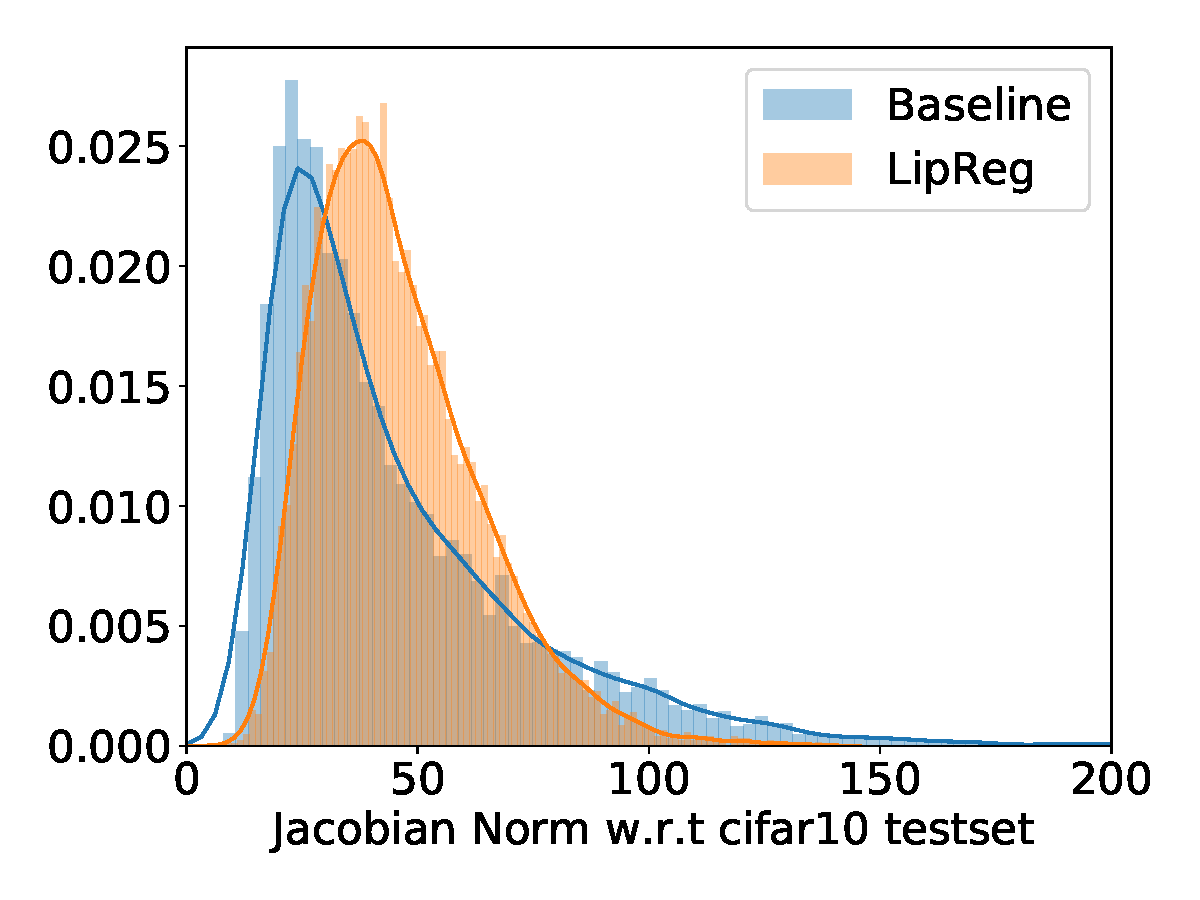
\includegraphics[width=\textwidth]{figures/part2/ch10-lipschitz_bound_adversarial/jacobian_distribution_v1.pdf}\\(a)
   \end{subfigure}
   \hfill
   \begin{subfigure}[b]{0.49\textwidth}
       \centering
       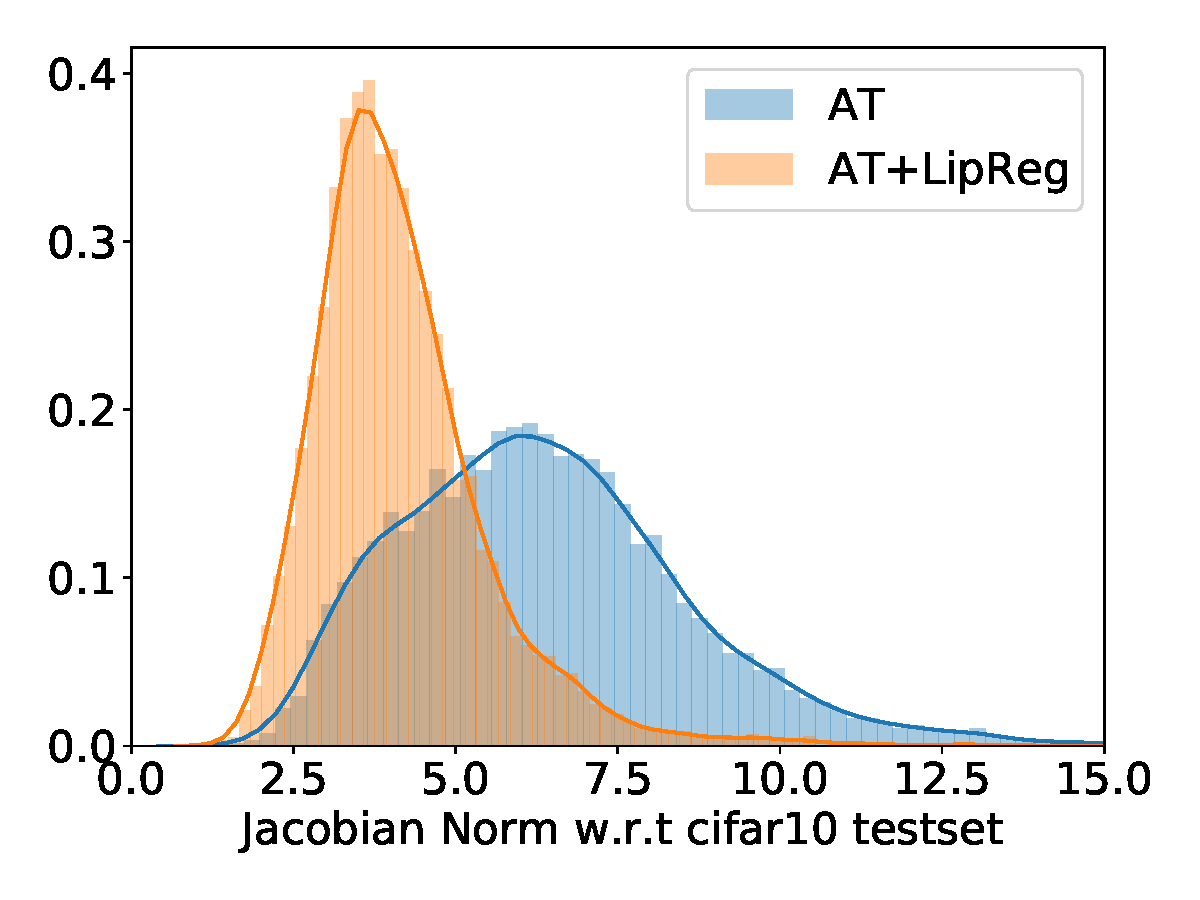
\includegraphics[width=\textwidth]{figures/part2/ch10-lipschitz_bound_adversarial/jacobian_distribution_v2.pdf}\\(b)
   \end{subfigure}
   \caption{These figures show the distribution of the norm of the Jacobian matrix w.r.t the CIFAR10 test set from a Wide Resnet trained with different schemes. Although Lipschitz regularization is not a Jacobian regularization, we can observe a clear shift in the distribution. This suggests that our method does not only work layer-wise, but also at the level of the entire network.}
   \label{figure:jacobian_distribution}
\end{figure}


\begin{figure}[ht]
   \centering
   \begin{subfigure}[b]{0.49\textwidth}
       \centering
       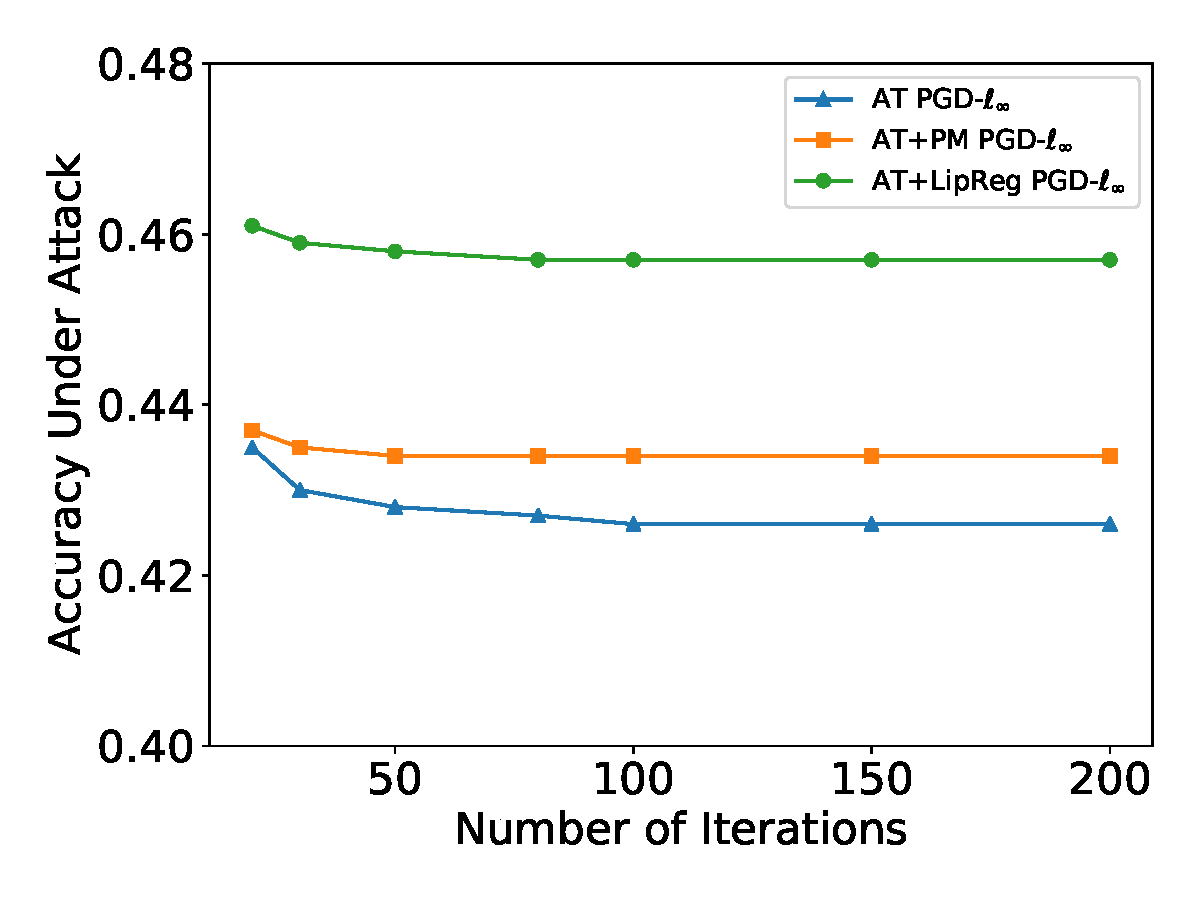
\includegraphics[width=\textwidth]{figures/part2/ch10-lipschitz_bound_adversarial/attacks_iter_pgd.pdf}\\(a)
   \end{subfigure}
   \hfill
   \begin{subfigure}[b]{0.49\textwidth}
       \centering
       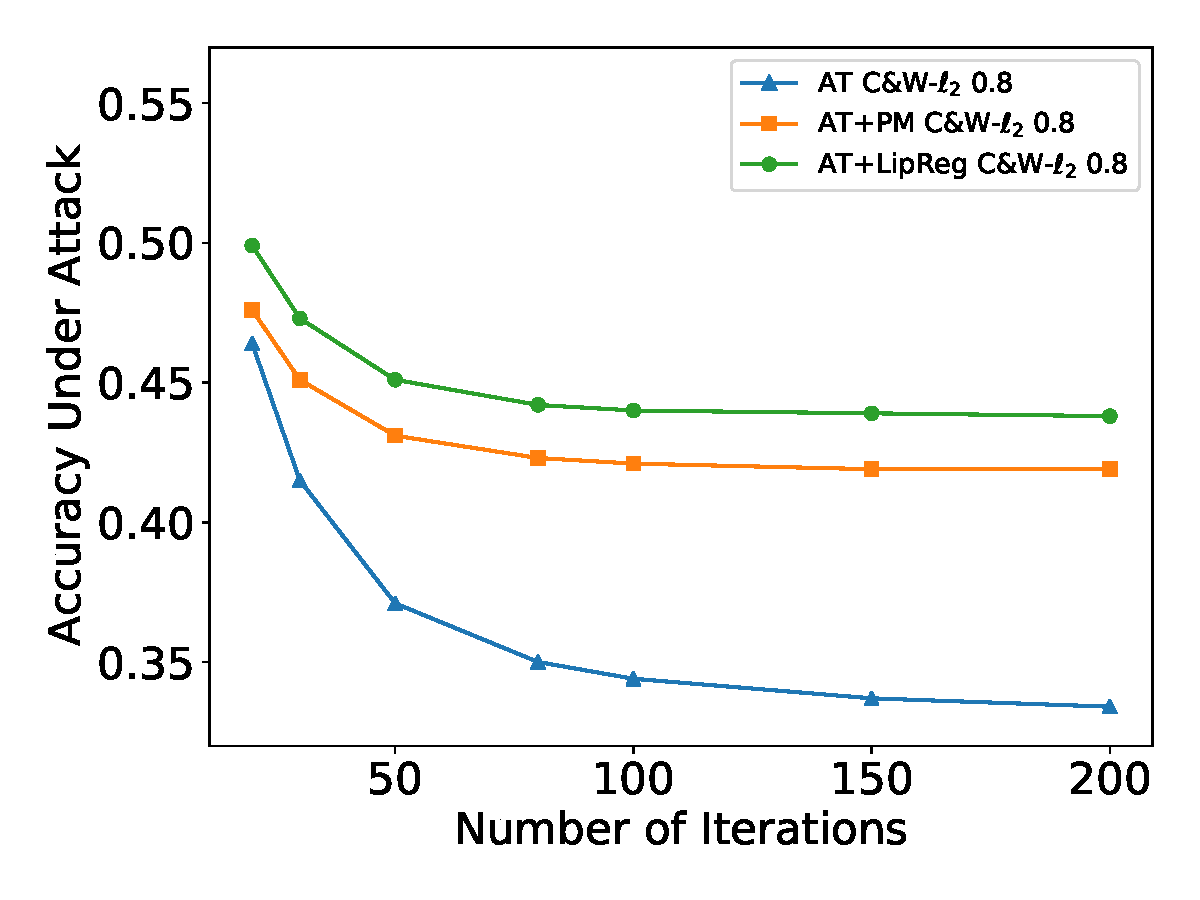
\includegraphics[width=\textwidth]{figures/part2/ch10-lipschitz_bound_adversarial/attacks_iter_cw.pdf}\\(b)
   \end{subfigure}
   \caption{These figures show the Accuracy under attack on CIFAR10 test set with PGD-$\linf$ and C\&W-$\ltwo$ attacks for several classifiers trained with Adversarial Training given the number of iterations.}
   \label{figure:attacks_iter}
\end{figure}


% \begin{figure*}[htb]
%   \centering
%   \begin{minipage}{.24\linewidth}
%     \centering
%     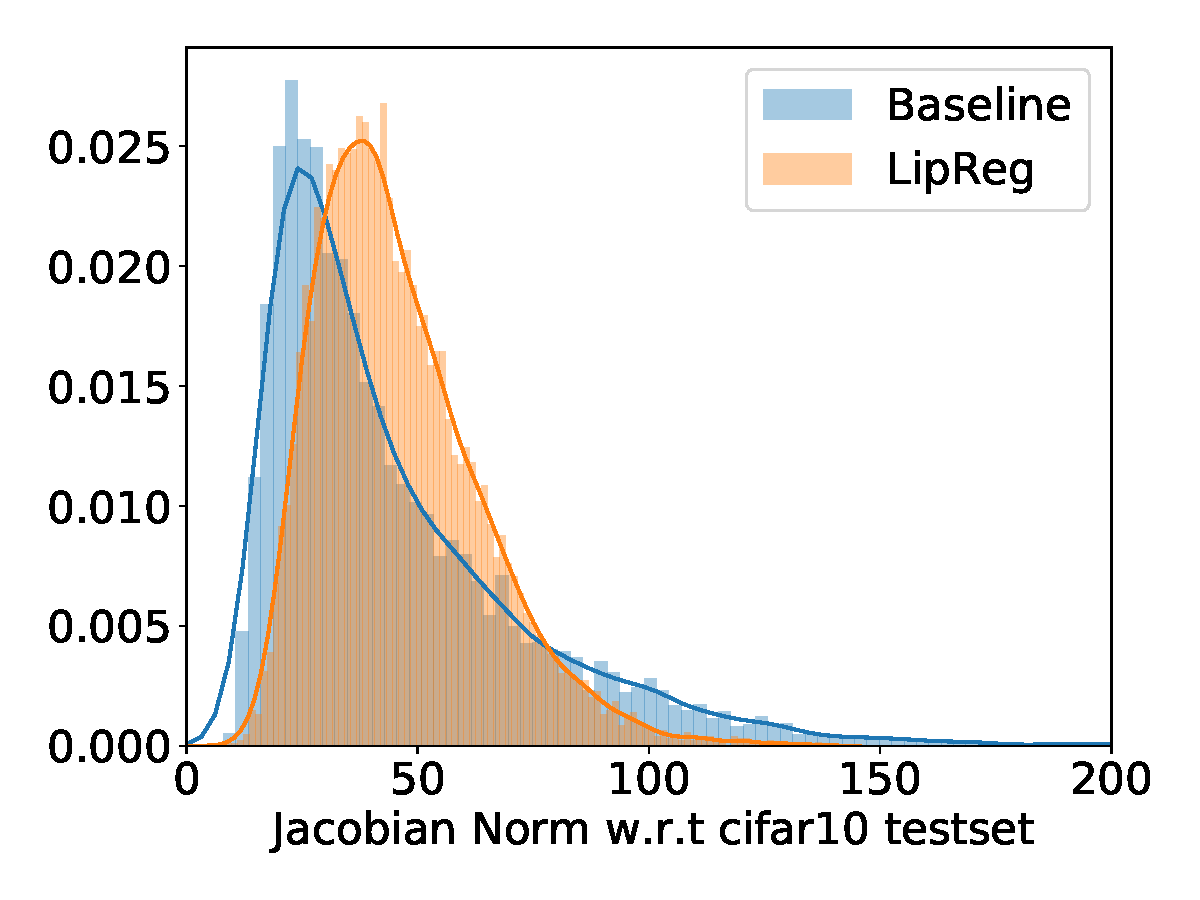
\includegraphics[scale=0.16]{figures/part2/ch10-lipschitz_bound_adversarial/jacobian_distribution_v1.pdf}\\{(a)}
%   \end{minipage}
%   \hfill
%   \begin{minipage}{.24\linewidth}
%     \centering
%     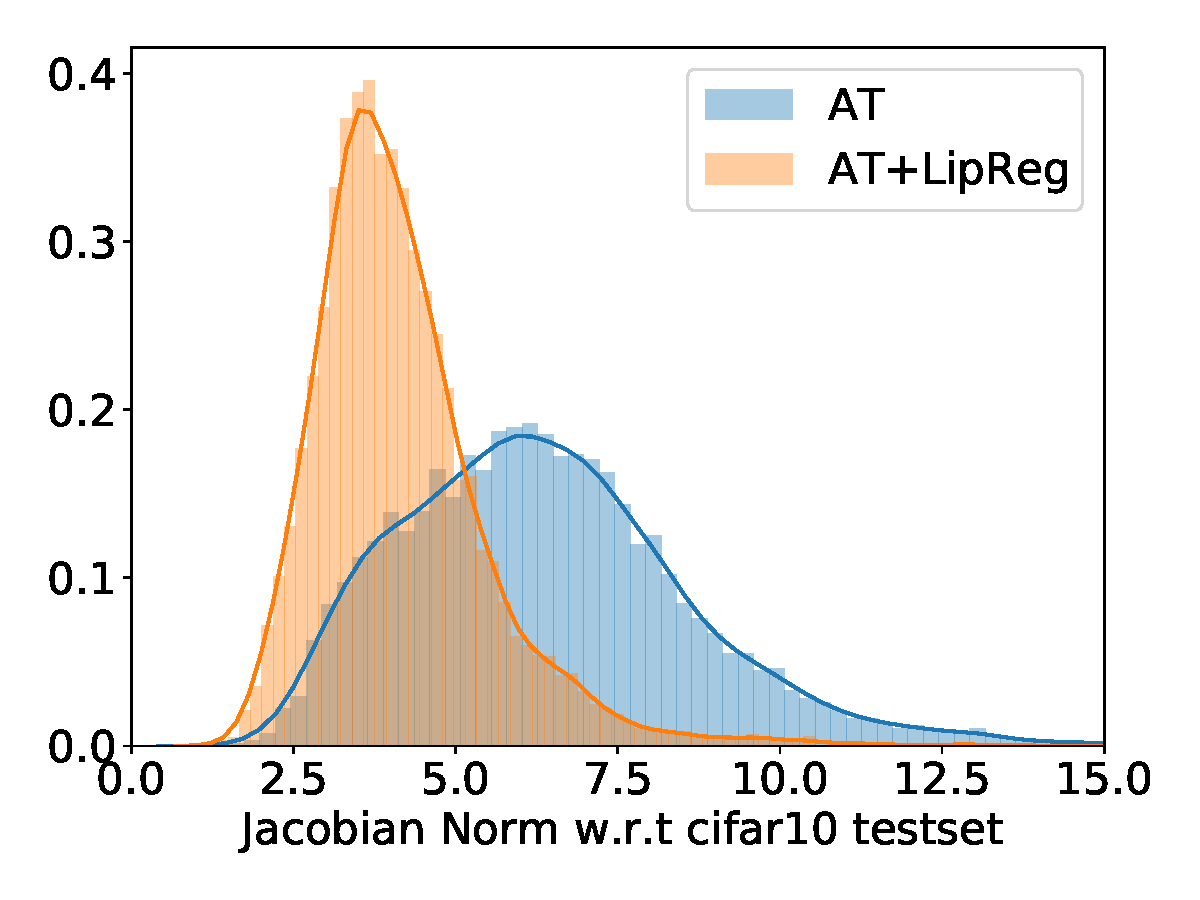
\includegraphics[scale=0.16]{figures/part2/ch10-lipschitz_bound_adversarial/jacobian_distribution_v2.pdf}\\{(b)}
%   \end{minipage}
%   \hfill
%   \begin{minipage}{.24\linewidth}
%     \centering
%     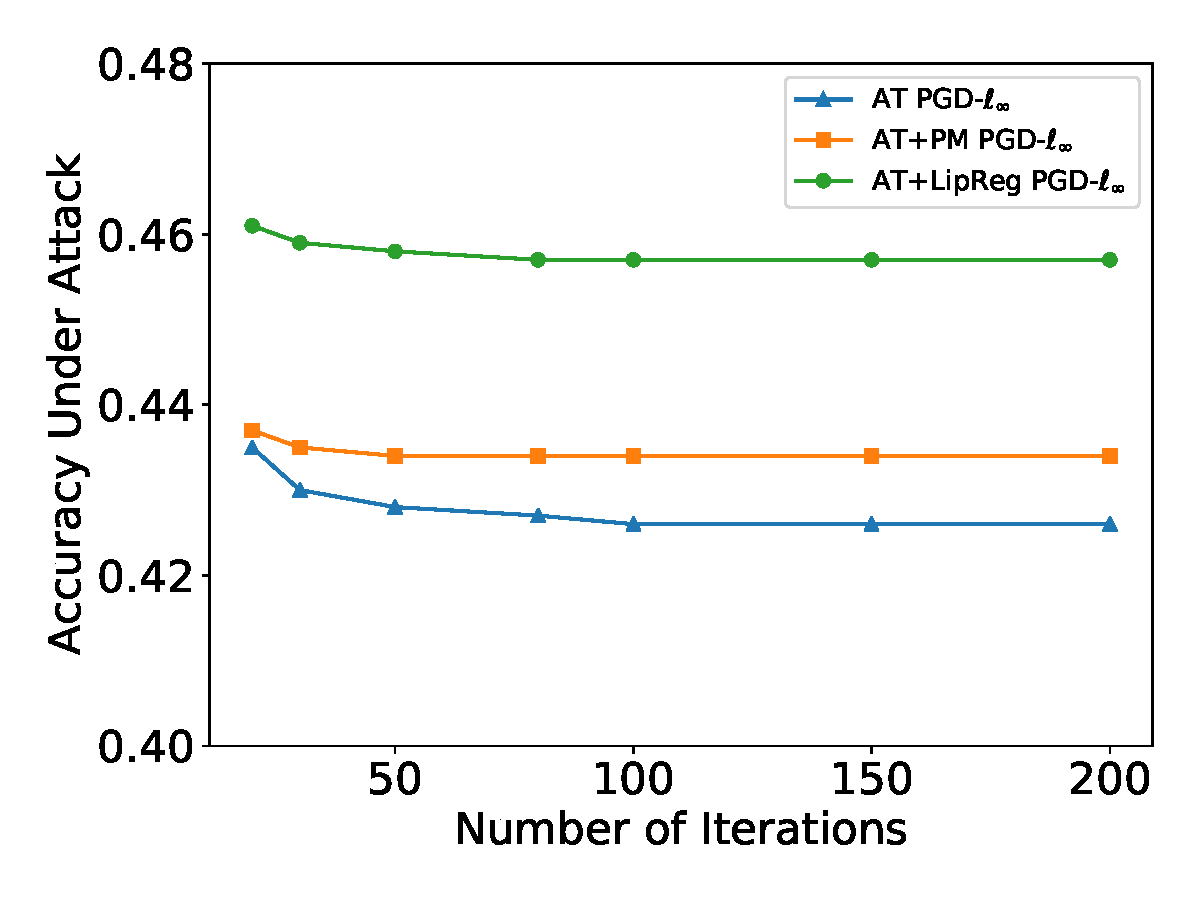
\includegraphics[scale=0.16]{figures/part2/ch10-lipschitz_bound_adversarial/attacks_iter_pgd.pdf}\\{(c)}
%   \end{minipage}
%   \hfill
%   \begin{minipage}{.24\linewidth}
%     \centering
%     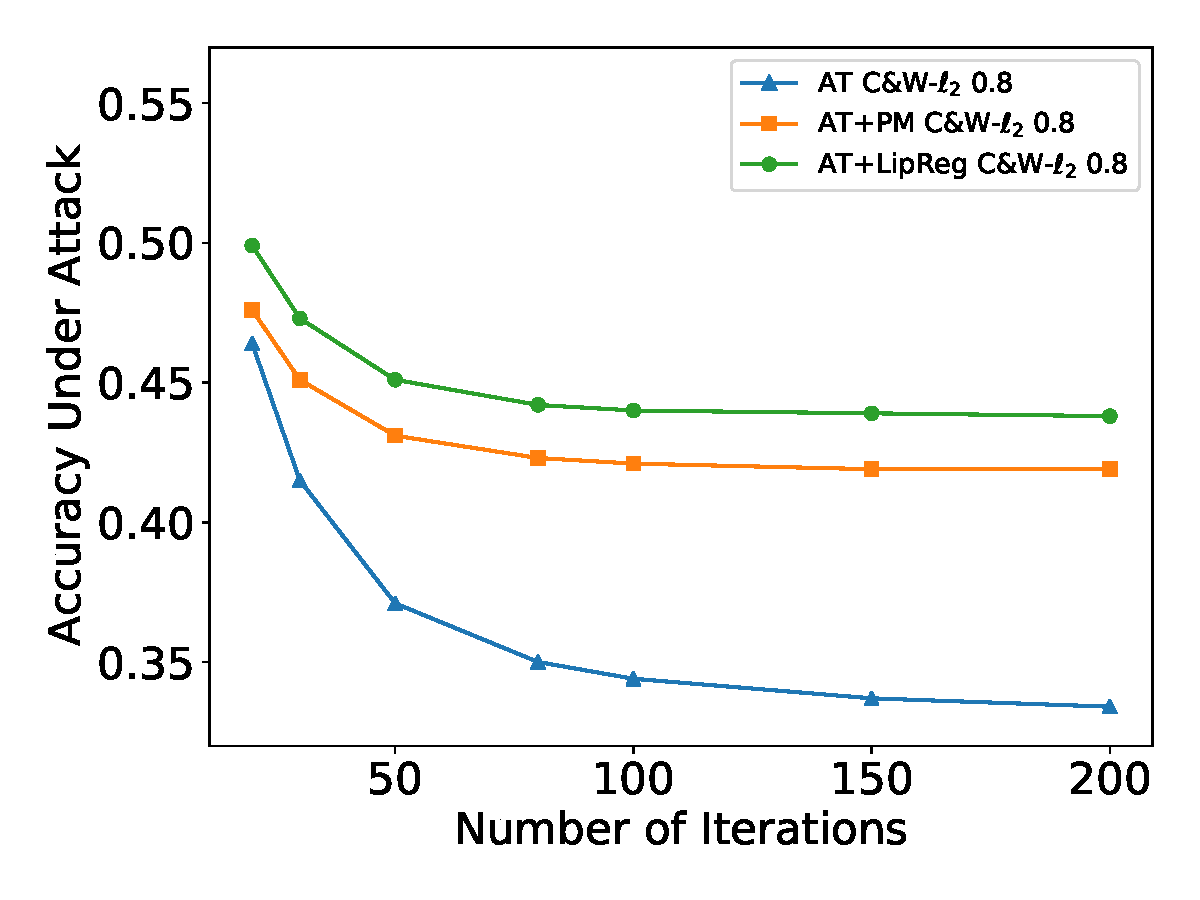
\includegraphics[scale=0.16]{figures/part2/ch10-lipschitz_bound_adversarial/attacks_iter_cw.pdf}\\{(d)}
%   \end{minipage}
%   \caption{Figures (a) and (b) show the distribution of the norm of the Jacobian matrix w.r.t the CIFAR10 test set from a Wide Resnet trained with different schemes. Although Lipschitz regularization is not a Jacobian regularization, we can observe a clear shift in the distribution. This suggests that our method does not only work layer-wise, but also at the level of the entire network. Figures (c) and (d) show the Accuracy under attack on CIFAR10 test set with PGD-$\linf$ and C\&W-$\ltwo$ attacks for several classifiers trained with Adversarial Training given the number of iterations.}
%   \label{figure:dist_jacobian_attacks_iter}
% \end{figure*}%


In this section, we compare the robustness of Adversarial Training~\cite{goodfellow2014explaining, madry2018towards} against the combination of Adversarial Training and Lipschitz regularization.
To regularize the Lipschitz constant of the network, we use the objective function defined in Equation~\ref{equation:objectif_function}.
We train Lipschitz regularized neural network with LipBound (Theorem~\ref{theorem:bound_max_sv_convolution}) implemented with PolyGrid (Algorithm~\ref{algorithm:PolyGrid}) (AT+LipBound) with $S = 10$ or with the specific power method for convolutions introduced by~\citet{farnia2018generalizable} with 10 iterations (AT+PM). 

Table~\ref{tab:table_cifar10_robustness} shows the gain in robustness against strong adversarial attacks.
We can observe that both AT+LipBound and AT+PM offer a better defense against adversarial attacks and that AT+LipBound offers a further improvement over the Power Method.
The Figure~\ref{figure:attacks_iter} (b) shows the Accuracy under attack with different number of iterations. 

Finally, we also conducted an experiment to study the impact of the regularization on the gradients of the whole network by measuring the norm of the Jacobian matrix, averaged over the inputs from the test set.
The results of this experiment are presented in Figure~\ref{figure:jacobian_distribution} (a) and show more concentrated gradients with Lipschitz regularization, which is the expected effect.
This suggests that our method does not only work layer-wise, but also at the level of the entire network.
A second experiment, using Adversarial Training, presented in Figure~\ref{figure:jacobian_distribution} (b) demonstrates that the effect is even stronger when the two techniques are combined together.
This corroborates the work by~\cite{farnia2018generalizable}.
It also demonstrates that Lipschitz regularization and Adversarial Training (or other Jacobian regularization techniques) are complementary.
Hence they offer an increased robustness to adversarial attacks as demonstrated above.

\paragraph{Experimental Settings}
We use the Wide ResNet architecture introduced by~\citet{zagoruyko2016wide} to train our classifiers (for details of the hyper-parameters used, see the supplementary material).
For Adversarial Training ~\cite{madry2018towards}, we use Projected Gradient Descent with an $\epsilon = 8/255 (\approx 0.031)$, a step size of $\textstyle \frac{\epsilon}{5} (\approx 0.0062)$ and 10 iterations, we use a random initialization but run the attack only once.
To evaluate the robustness of our classifiers, we rigorously followed the experimental protocol proposed by~\citet{tramer2020adaptive} and~\citet{carlini2019evaluating}.
More precisely, as an $\linf$ attack, we use PGD with the same parameters ($\epsilon = 8/255$, a step size of $\textstyle \frac{\epsilon}{5}$) but we increase the number of iterations up to 200 with 10 restarts.
For each image, we select the perturbation that maximizes the loss among all the iterations and the 10 restarts.
As $\ltwo$ attacks, we use a bounded version of the~\cite{carlini2017towards} attack.
We choose $0.6$ and $0.8$ as bounds for the $\ltwo$ perturbation. Note that the $\ltwo$ ball with a radius of $0.8$ has approximately the same volume as the $\linf$ ball with a radius of $0.031$ for the dimensionality of CIFAR10. 


\subsection{Results on CIFAR100 dataset \& Hyper-parameters}

\begin{table}[htb]
  \centering
  \caption{This table shows the Accuracy under $\ltwo$ and $\linf$ attacks of CIFAR100 dataset. We compare Adversarial Training with the combination of Lipschitz regularization and Adversarial Training \cite{madry2018towards}. The $\lambda_2$ parameters which control the Lipschitz regularization is $0.008$, it has been chosen among a grid search of 10 values. The attacks below are computed with 200 iterations.}
    \begin{tabular}{lcccc}
    \toprule
      & \textbf{Accuracy} & \textbf{PGD-$\linf$} & \textbf{C\&W-$\ltwo$ 0.6} & \textbf{C\&W-$\ltwo$ 0.8} \\
    \midrule
    \textbf{Baseline} & $\mathbf{0.792}\pm0.000$ & $\phantom{.}0.000\pm0.000$ & $\phantom{.}0.001\pm0.000$ & $\phantom{.}0.000\pm0.000$ \\
    \textbf{AT} & \phantom{.}$0.591\pm0.000$ & $\phantom{.}0.199\pm0.000$ & $\phantom{.}0.263\pm0.000$ & $\phantom{.}0.183\pm0.000$ \\
    \textbf{AT+LipReg} & \phantom{.}$0.552\pm0.019$ & $\mathbf{0.215}\pm0.004$ & $\mathbf{0.294}\pm0.010$ & $\mathbf{0.226}\pm0.008$ \\
    \bottomrule
    \end{tabular}%
  \label{tab:results_cifar100}%
\end{table}%


\paragraph{Hyper-parameters used for training classifiers on CIFAR10 \& CIFAR100 dataset}
For all our experiments, we use the Wide Resnet architecture \cite{zagoruyko2016wide} with 28 layers and a width factor of 10. We train our networks for 200 epochs with a batch size of $200$. We use Stochastic Gradient Descent with a momentum of $0.9$, an initial learning rate of $0.1$ with exponential decay of 0.1 (MultiStepLR gamma = 0.1) after the epochs $60$, $120$ and $160$. 

\subsection{Results on ImageNet dataset \& Hyper-parameters}

\begin{table}[htb]
  \centering
  \caption{This table shows the accuracy and accuracy under attack of ImageNet dataset with different training schemes. We compare Adversarial Training with the combination of Lipschitz regularization and Adversarial Training \cite{madry2018towards}. }
    {\footnotesize
    \begin{tabular}{lccccccccc}
    \toprule
      & \multicolumn{1}{c}{\multirow{2}[4]{*}{$\lambda_2$}} & \multicolumn{1}{c}{\multirow{2}[4]{*}{\textbf{Natural}}} &   & \multicolumn{2}{c}{\textbf{PGD-}$\linf$} &   & \multicolumn{3}{c}{\textbf{C\&W-}$\ltwo$} \\
\cmidrule{5-6}\cmidrule{8-10}      &   &   &   & \multicolumn{1}{c}{0.02} & \multicolumn{1}{c}{0.031} &   & \multicolumn{1}{c}{1.00} & \multicolumn{1}{c}{2.00} & \multicolumn{1}{c}{3.00} \\
    \midrule
    \textbf{AT} & \multicolumn{1}{c}{-} & 0.509 &   & 0.251 & 0.118 &   & 0.307 & 0.168 & 0.099 \\
    \textbf{AT+LipReg} & 0.0006 & \textbf{0.515} &   & \textbf{0.255} & \textbf{0.121} &   & \textbf{0.316} & \textbf{0.177} & \textbf{0.105} \\
    \textbf{AT+LipReg} & 0.0010 & \textbf{0.519} &   & \textbf{0.259} & \textbf{0.123} &   & \textbf{0.338} & \textbf{0.204} & \textbf{0.129} \\
    \bottomrule
    \end{tabular}%
    }
\end{table}%


\paragraph{Hyper-parameters used for training and attacking classifiers on ImageNet dataset}

For all our experiments, we use the Resnet-101 architecture \cite{he2016deep}.
We have used Stochastic Gradient Descent with a momentum of $0.9$, a weight decay of $0.0001$, label smoothing of $0.1$, an initial learning rate of $0.1$ with exponential decay of $0.1$ (MultiStepLR gamma = $0.1$) after the epochs $30$ and $60$.
We have used Exponential Moving Average over the weights with a decay of $0.999$.
We have trained our networks for 80 epochs with a batch size of $4096$.
For Adversarial Training, we have used PGD with 5 iterations, $\epsilon = 8/255 (\approx 0.031)$ and a step size of $\frac{\epsilon}{5} (\approx 0.0062)$. 

To evaluate the robustness of our classifiers in ImageNet, we have used an $\linf$ and an $\ltwo$ attacks. More precisely, as an $\linf$ attack, we use PGD with an epsilon of 0.02 and 0.031, a step size of $\textstyle \frac{\epsilon}{5}$) but we increase the number of iterations to 30 with 5 restarts. For each image, we select the perturbation that maximizes the loss among all the iterations and the 10 restarts. As $\ltwo$ attacks, we use a bounded version of the~\cite{carlini2017towards} attack. We have used $1$, $2$ and $3$ as bounds for the $\ltwo$ perturbation. 





